\documentclass[12pt,a4paper]{extarticle}
\usepackage{hyperref}
\usepackage{amsmath,amsthm,amssymb,scrextend,enumerate}
\usepackage[utf8]{inputenc}
\usepackage{graphicx}
\usepackage{pgfplots}
\linespread{1.5}

\title{COMP2610 Summary}
\begin{document}
\maketitle
\tableofcontents
\section{Others}
** Approximate to $3^{rd}-4^{th}$ decimal number.\\
** "Assuming", "if", "given", "for" are key words for identify conditions.\\
** Be careful the $99 \% = 0.99$ but $\frac{999}{1000} \neq 99\%$\\
** Translate and write notation/formula at first. Then find the given conditions.\\
** Be careful the text number conditions\\
** Write in $log_2$

\section{Basic}
$(log_2(x))'=\frac{1}{x\ln(2)}$ \quad $(log_2(1-x))'=-\frac{1}{(1-x)\ln(2)}$\\                                                                                                                                                                                                                                                                                                                                                                                                                                                                                                                                                                                                                                                                                                                                                                                                                                                                                                                                                                                                                                                                                                                                                                                                                                                                                                                                                                                                                                                                                                                                                                                                                                                                                                                                                                                                                                                                                                                                                                                                                                                                                                                                                                                                                                                                                                                                                                                                                                                                                                                                                                                                                                                                                                                                                                                                                                                                                                                                                                                                                                                                                                                                                                                                                                                                                                                                                                                                                                                                                                                                                                                                                                                                                                                                                                                                                                                                                                                                                                                                                                                                                                                                                                                                                                                                                                                                                                                                                                                                                                                                                                                                                                                                                                                                                                                                                                                                                                                                                                                                                                                                                                                                                                                                                                                                                      
\textbf{Marginal} $p(X)$\\
\textbf{Joint} $p(X,Y)$\\
\textbf{Conditional} $p(X|Y)$\\
\newline
\textbf{Marginal Distribution}\\
$p(X) = \sum_jp(X=x_i,Y=y_j)$(Law of Total Probability)\\
$p(Apple)=p(Apple,r)+p(Apple,g)+p(Apple,b)=p(Apple|r)p(r)+p(Apple|g)p(g)+p(Apple|b)p(b)$\\
\newline
If $X \perp Y$ (X and Y are independent random variables):\\$p(X,Y)=p(X)p(Y)$\\
\newline
\textbf{Conditional}\\
If $X \perp Y$ (X and Y are independent random variables):\\$p(X|Y)=p(X)$\\
$p(Coin = HH|Fair) = p(H|Fair)*p(H|Fair)$\\
If X is binary $\{0,1\}$ then $p(X=1|Y=1)= 1-p(X=0|Y=1)$\\
\newline
\textbf{Product Rule}\\
$p(A,B)=p(A|B)p(B)=p(B|A)p(A)$\\
$p(A|B)$ \& $p(B|A)$ can use above formula or Bayesian Rule\\
\newline
\textbf{Bayesian Rule}\\
$p(X|Y)=\frac{p(Y|X)p(X)}{p(Y)}$\\
Posterior:$p(X|Y)$ \quad Prior(uncertain quantity):$p(X)$ \quad Likelihood: $p(Y|X)$ \\
Prior $\uparrow$, then Posterior $\uparrow$, they are proportional\\
Use to calculate the fraction of a probability.\\
Prior: what we believe X is likely to be \textbf{before} looking at the data\\
Posterior: what we believe X is likely to be \textbf{after} looking at the data.\\
\newline 
\textbf{Expetation}\\
$E[X] = \sum_{x\in \{X\}} p(x)*x$\\
$E[X|Y=y]=\sum_{x\in \{X\}} p(X=x|Y=y)*x$\\
$E[XY]=\sum_{x=0}^1 \sum_{y=-1}^1 p(X=x,Y=y)*x*y$\\
$Var(X)= E[X^2]-E[X]^2$\\
$Cov(X,Y)=E[XY]-E[X]E[Y]$ Cov is the correlation coefficient\\
\textbf{Cox Axioms}\\
Given B(x), B($\bar{X}$), B(X,Y), B(Y):\\
* Degree of belif can be ordered\\
*$B(X)=f[B(\bar{x})]$\\
*$B(X,X)=g[B(X|Y),B(Y)]$\\

\section{Bernoulli, Binomial, Max Likelihood, MAP}
\textbf{Bernoulli Distribution}\\
Variable has outputs $\{0,1\}$\\
$p(X=1|\theta)=\theta$ \quad $p(X=0|\theta)=1-\theta$\\
$p(X=x|\theta)=\theta ^x (1-\theta)^{1-x}$\\
Expected Value(Mean): $E[X|\theta]=\sum_{x\in X} p(x|\theta)*x=N\theta$\\
Variance(SquareStandard Deviation): $V[X|\theta]=E[(X-E[X])^2]=N\theta(1-\theta)$\\
\newline
\textbf{Binomial Distribution}\\
Distributions of Bernoulli variables\\
Expected Value(Mean): $E[Y]=\sum_{m=0}^N Bin(m|N,\theta)=N\theta$\\
Variance(SquareStandard Deviation): $V[X|\theta]=\sum_{m=0}^N(m-E[m])^2Bin(|N,\theta)=N\theta(1-\theta)$\\
$p(Y=m)=Bin(m|N,\theta)=\binom{N}{m}\theta^m(1-\theta)^{N-m}$\\
Num of ways get m heads out of N coin flip:$\binom{N}{m}=\frac{N!}{(N-m)!m!}$\\
$Binomial(x; n, P) = nCx * P^x * (1 - P)^{n - x} $ X: value; n: $\# times$; p:probability \\
$nCx = \frac{n!}{(n-x)!x!}$\\
\newline
\textbf{Parameter Estimation}\\
According to sequence D $\{0/1\}$:\\
$\begin{cases}
 & \text{ if } D[i]=1 \quad p(x_i|\theta)=(1-\theta)\\ 
 & \text{ if } D[i]=0 \quad p(x_i|\theta)=\theta
\end{cases}$\\
Maximum Likelihood Estimator(MLE)$\hat{\theta} =\arg max_\theta L(\theta|x)$\\
Likelihood Function(probability of a sequence): $L(\theta)=p(D|\theta)=\prod ^{10}_{i=1}p(x_i|\theta)=\prod^N_{i=1}\theta^{x_i}(1-\theta)^{1-x_i}$\\
Maximum Likelihood(maxing likelihood): $\mathcal{L}(\theta)=log(p(D|\theta))=\sum^N_{i=1}log p(x_i|\theta)=\sum^N_{i=1}[x_ilog\theta + (1-x_i)log(1-\theta)]$\\
** Max likelihood uses $\sum$ and $log$, while likelihood uses $\prod$.\\
$\theta_{ML}=\frac{1}{N}\sum^N_{i=1}x_i$\\
\newline
\textbf{Beta Prior}\\
The likelihood of X given $\theta$: Bern$(X=x|\theta)=\theta ^x (1-\theta)^{1-x}$\\
prior (Beta Distribution):Beta$(\theta|a,b)= \frac{1}{Z(a,b)}\theta^{a-1}(1-\theta)^{b-1}$\\
Z(a,b) is a suitable normaliser.\\
posterior(By using Beta prior): $p(\theta|D,a,b)=\frac{p(D|\theta)p(\theta|a,b)}{p(D|a,b)}=Beta(\theta|m+a,l+b)$\quad $m=x$; $l = 1-x$\\
If more data are coming, this posterior will become the new prior of next round.\\
Maximum A Posterior(MAP) uniform distribution: $\theta_{MAP}=\frac{m+a-1}{N+a+b-2}$\\
Maxim Likelihood: $\theta_{ML}=\frac{m}{N}$ not like max likelihood of Bernoulli model, it doesn't use prior.\\
If a=b=1, then $\theta_{MAP}=\theta_{ML}$\\


\section{Entropy}
how informative is a  message?\\
information content(outcome of x):$h(x)=log_2\frac{1}{p(x)}$ (unit in bits)\\
average information content of outcome: $H(X)= E_x[h(X)]\geq 0$\\
average information length: $\sum^N_{i=1} p_i(X)*N*l$ \quad N:Num of this probability, l:Num of bit X used. (unit in bits)\\ 
$H(X)=\sum_{x\in {x_1,x_2,x..}} p(X)log_2 (\frac{1}{p(X)})=-\sum_{x\in {x_1,x_2,x..}} p(X)log_2 (p(X))$\\
$H(X|\ Y)= \sum_{y\in {y_1,y_2,y..}} H(X|Y=y)\cdot p(Y=y) $; $y\in Y$ is known; $H(X|Y=0)=H(p(x1|y=0),p(x2|y=0),....)=H(p(x1,y=0)/p(y=0),p(x2,y=0)p(y=0),....)=$ sum up all $p(x|y=0)log_2\frac{1}{p(x|y=0)}$\\
Entropy is maximised if p peaked; entropy is minimised if p uniformly distributed.\\
If p is \textbf{uniform} $\frac{1}{|X|}$, entropy is maximised. If p is uniform, then $H(X)= log_2(X)$ \quad $log_2|X|$ is the Num of bits needed to describe an outcome of X.\\
If not uniform, use shorter codes for object with higher probability, use longer codes for object with lower probability.\\
Entropy is the lower bound on average number of bits.\\
Adding outcomes of probability 0 does not affect H.\\
\newline
\textbf{Joint Entropy}\\
$H(X,Y)=E_{X,Y}[log\frac{1}{p(X,Y)}]=\sum_{x\in X} \sum_{y\in Y} p(x,y)log\frac{1}{p(x,y)}$\\
By chain rule: $H(X,Y)=-\sum_{x\in X}\sum_{y\in Y}p(x,y)log(p(x,y))=
-\sum_{x\in X}\sum_{y\in Y}p(x,y)[log(p(x))+log(p(y|x))]$\\
$H(X,Y)=H(X)+H(Y|X)=H(Y)+H(X|Y)$\\
The joint uncertainty of X and Y is the uncertainty of X plus the uncertainty of Y given X.\\
If $X \perp Y$ (X and Y are independent random variables):H(X,Y)=H(X)+H(Y)\\
\newline
\textbf{Conditional Entropy}\\
Entropy of the probability distribution $p(X|Y=y)$: $H(X|Y=y)=\sum_{x\in X} p(x|Y=y)log \frac{1}{p(x|Y=y)}$\\
The average over Y of the conditional entropy X given Y=y: $H(X|Y)=\sum_{y\in Y} p(y)H(X|Y=y)=\sum_{y\in Y}p(y)\sum_{y\in Y}p(y|x)log\frac{1}{p(x|y)}=\sum_{x\in X}\sum_{y\in Y}p(x,y)log(\frac{1}{p(x|y)})=E_{x,y}[log(\frac{1}{p(X|Y)})]$\\
\section{Kullback-Leibler(KL) Divergence}
$D_{KL}(p||q)=\sum_{x\in X}p(x)(log\frac{1}{q(x)}-log\frac{1}{p(x)})=\sum_{x\in X} p(x)log(\frac{p(x)}{q(x)})=E_{p(x)}[log(\frac{p(x)}{q(x)})]$\\
If q uniform, $q(x)= \frac{1}{|X|}$:\quad $D_{KL}(p||q)=\sum_{x\in X} p(x)log(\frac{p(x)}{q(x)})= \sum_{x\in X}p(x)(log(p(x))+log|X|)=-H(X)+log|X|$\\
If p=q(symmetry), $D_{KL}(p||q)=D_{KL}(q||p)$\\


\section{Mutual Information}
$I(X;Y)\geq 0$\\
Since all mutual information is symmetry, $I(X;Y)=I(Y;X)$\\
Self Information: I(X;X)= H(X)\\
$I(X;Y)=D_{KL}(p(X,Y)||p(X)p(Y))=\sum_{x\in X}\sum_{y\in Y}p(x,y)log(\frac{p(x,y)}{p(x)p(y)})$\\
$I(X;Y)=H(X)-H(X|Y)=H(Y)-H(Y|X)=H(X)+H(Y)-H(X,Y)$\\
If $X \perp Y$ (X and Y are independent random variables):I(X;Y)=0\\
The mutual info btw X and Y given $Z=z_k$: $I(X;Y|Z=z_k)=H(X|Z=z_k)-H(X|Y,Z=z_k)=E_{p(x,y,z)}log(\frac{p(X,Y|Z)}{p(X|Z)p(Y|Z)})$\\
I(X;Y,Z)=$I(X;Y)+I(X;Z|Y)=I(X;Z)+I(X;Y|Z)$\\
$I(X,Y;Z) \neq I(X;Y,Z)$(Most of cases) but $I(X;Y,Z)=I(Y,Z;X)=I(X;Z)+I(X;Y|Z)=I(X;Y)+I(X;Z|Y)$\\

\begin{figure}
  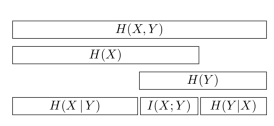
\includegraphics{img/lec7-0}
  \caption{lec07-0}
  \label{fig:lec07-0}
\end{figure}

\section{Convex Functions}
$f(\lambda X_1+(1-\lambda)X_2)\leq \lambda f(X_1)+(1-\lambda)f(X_2)$\\
If $\lambda = \{0,1\}$, $f$ is strictly convex\\
* concave: $\frown$ \quad convex: $\smile$\\
If concave, there is a point: $\frac{df}{dx}=0$ (Maximum point); But the derivative is not the Must condition that shows there is a max point.\\


\section{Inequality}
\textbf{Jensen's Inequality}\\
convex: $\smile$: $f(E[X])\leq E[f(X)]$ verse versa.\\
\newline
\textbf{Gibbs's Inequality}\\
$D_{KL}(p||q)\geq 0$if p(x)=q(x)\\
If $X\perp Y$: $I(X;Y)=D_{KL}(p(X,Y)||p(X)p(Y))\geq 0$\\
If $X\perp Y$: $H(X|Y)\leq H(X)$ ($I(X;Y)\geq 0$)Data don't increase uncertainty on average, info cannot hurt on average.\\
discret variable X: $H(X)\leq log|X|$
\newline
\textbf{Large Number}\\
Independent distribution\\
$E[X_i]=\mu$ and $\ overline{x}_n=\frac{X_1+...+X_n}{n}$ $lim_{n\to\infty}p(|\overline{X}_n-\mu|>\epsilon)=0$\\
$V[\overline{X}_n]=\frac{V[X_1+..+X_n]}{n^2}=\frac{n\sigma^2}{n^2}$
\newline
\textbf{Markov's Inequality}\\
Markov Chain: $p(X,Y,Z)=p(X)p(Y|X)p(Z|Y)$, it gives $X\perp Z|Y \Rightarrow p(X|Y,Z)=p(X|Y)$\\ 
(1) X and Z are conditional independent given Y;\\
(2)If Z=f(Y), then $X\to Y\to Z$, then $I(X;Y)\geq I(X;f(Y))$\\
(3)$X\to Y\to Z$ implies $Z\to Y\to X$\\
(4)If $X\to Y\to Z$, then $I(X;Y)\geq I(X;Z)$\\
Eatimate the MAX possible number of students who scored more than 80.\\
(1)Bound: $p(X\geq \lambda)\leq \frac{E[X]}{\lambda}$e.g. $\lambda < E[X]$ and $0<\lambda <1$ E[X]=n*P(X)\\
Only use mean of distribution\\
The bound from Markov's inequality $A$ be within $1\%$ of exact probability $B$:
$A-B=1\%$\\
\newline
\textbf{Chebychev's Inequality}\\
$p(|X-E[X]|\geq \lambda \sqrt{V[X]})\leq \frac{V[X]}{(\lambda \sqrt{V[X]})^2} \leq \frac{1}{\lambda^2}$\\
\section{Ensembles}
Ensemble X $\in \{x,A_x,P_x\}\{\text{Random Value, Values, Probability}\}$;\\
$H(X^N)=NH(X)$\\
Probability of types: $P(x)=p_1^{n_1}*p_2^{n_2}*...  $\\
$\#$ of sequence with $n_i$ copies of $a_i= \frac{N!}{n_1!n_2!...}$\\
$N*p_x$: expectation of most likely sequence (single sequence has all same variables e.g. p(hhhh)).\\
Variation is small when $\beta$(clossness) is small.\\
$\#$ of sequences in the typical set: $T_{N\beta}\leq 2^{N(H(X)+\beta)}$; If binary low entropy: $T_{N\beta}\leq 2^{N(H(X)+\beta)}<<2^N$\\
$H(X)-\beta <-\frac{1}{N}log_2P(k)<H(X)+ \beta$\\
For large X: $H(X)-\delta < \frac{1}{N}H_\delta (X^N)$; H(X) is the boundary\\
The most likely sequence may not belong to the typical set.\\
\textbf{Asymptotic Equipartition Property AEP}\\
Almost all sequences are typical\\
Informal: $log_2 P(x_1,x_2....x_N)$ is close to $-NH(X)$ with high probability\\
If N large enough, it guarantees draw a sequence from a small set\\
If N larger, $S_\delta $ and $T_{N\beta}$ increasingly overlap. $|S_\delta|\leq T_{N\beta}$\\
If $<\beta$ $lim_{N\to \infty}p(...)=1$; If $>\beta$ $lim_{N\to \infty}p(...)=0$\\
Length of sequence $\uparrow$, the probability of "typical" sequence $\uparrow$ and larger than "atypical" sequence.
\section{Source Coding Theorem SCT}
If large sequence $\to$ average bits of each outcome = entropy of source\\
Average bit per outcome: $\sum l(x_i)p_i$\\
$p_i$ are the weight\\
Lossless/Unique Decode-ability for variable-length code:\\
$x\neq y \to c(x)\neq c(y)$ \quad Lossless: for outcomes; Unique Decodable: for string results\\
Prefix free $\Rightarrow$ Unique Decodable; Loss less $\neq$ Unique decodable \quad unique decodable $\neq$  prefix free $\quad$ \\
\newline
\textbf{Lossy Coding}\\
Raw Bit Content: $H_0(X)=log_2|A_x|$ $A_x$: $\#$ of outcomes. probability of outcomes are ignored\\
* Reliable Probability of N outcomes: $(1-p_{none})^N = 1-nCx*p(X=0)^{n-x}*p(X=1)^{x}$\\
* Expected Bit of N outcomes: $N\frac{\sum l(x_i)p_i}{1-p_{none}}=N$\\
* Lossless bit = xN (x: $\#$ of non-none code)\\
\newline
\textbf{Essential Bit Content}\\
* Essential Bit content: $H_\delta(X)=log_2|S_\delta|$ $S_
\delta $: $\#$ of elements in set\\
Trade off in \textbf{uniform lossy} code: define $S_\delta$ as smallest subset of $A_x$; $P(x\in S_\delta) \geq 1 - \delta $\\
If only uniformly code elements in $S_\delta$:\\ 
* Reliable Probability of N outcomes: $(1-
\delta)^N$\\
* Expected Bit of N outcomes: $Nlog_2|S_\delta|$\\
Set $\delta$ from 0, then to the smallest $p_i$, then 1 - smallest($p_i$) until no more left.
For \textbf{uniform code}:\\
There is a $N_0$ such that $N\geq N_0$: $|\frac{1}{N}H_\delta(X^N)-H|<\epsilon $\\
* Average bit in uniform code $\delta$ portion: $\frac{1}{N}H_\delta(X^N)$\\
Tiny probability of error $\delta \to$ close to H\\
large probability of error $\delta \to$ cannot compress more than H bits per symbol.\\
** Raw bit content: $H_\delta(X^4) \neq 4H_\delta(X)$ But entropy $H(X^4)=4H(X)$\\
Why curve is flat? $\because \delta \uparrow$ the quicker encounter sequence; It makes small and similar sized changes to $|S_\delta|$\\
If N $\uparrow \quad log_2|S_\delta| \approx NH$\\
If use $< NH(X)$ bits per block, then lose information\\
** Bad practical to perform coding, needs huge block size $N_0$ and look up tables size is huge.\\
\newline
\textbf{Kraft Inequality}\\
If there is a prefix code C , then any binary prefix this code C, its code length: $\sum^I_{i=1}2^{-l_i}\leq 1$\\
For Prefix Exclude Codes:\\
An l-bits codeword excludes $2^{k-l}*$k-bit codewords. e.g. 4*3-bit codewords:$\{000,001,010,...\}$\\
There are only $2^{l*}$ possible $l^*$-bit codewords\\
Remove descendants(tree like) once its root is chosen as the prefix. \\
Even given code length satisfy the Kraft Inequality, doesn't mean code itself is prefix, just mean the code of length can be used to be the standard length to construct prefix.\\
\newline
\textbf{Expected Code Length}\\
L(C,X)=$E[l(x)]=\sum_{x\in A_x}p(x)l(x)=\sum^l_{i=1}p_il_i$\\
Probability vector: $q_i = \frac{2^{-l_i}}{z}$; \quad  $z=\sum_i 2^{-l_i}$;\quad $l_i = log_2(\frac{1}{zq_i})$\\
Limited of Compression: $L(C,X)=H(X)+D_{KL}(p||q)+log_2\frac{1}{z}\geq H(X)$(with equality when $l_i=log_2\frac{1}{p_i}$)\\
q: probability of code length; p: probability of ensemble. p=q(Gibb's Inequality)\\
\newline
\textbf{Shannon Codes}\\
Shannon codes are suboptimal, don't need smallest expected length\\
$\lceil log_2\frac{1}{p_i}\rceil$\\
$H(X)\leq L(C,X)\leq H(X)+1$ \\
\newline
\textbf{Huffman Codes}\\
Huffman codes (prefix) are optimal. Find the smallest two to assign 0 and 1, then combine them in the next step. The non-combined will be kept in the next step.\\
$H(X)\leq L(C_{Huff},X)\leq L(C_{other},X)\leq H(X)+1$\\
Best sybol codes, but notthe best code.\\
\newline
\textbf{Shannon-Dano-Elias Codes}\\
Worse than Huffman, prefix free; if code lossless, then F(x-1)$<\lfloor \overline{F}(x)\rfloor _{l(x)}<\lfloor \overline{F}(x)\rfloor_{l(x)}+\frac{1}{2^l} <$ F(x)(don't overlap, guarantee interval)\\
Cumulative Distribution: $F(x)=\sum_{i\leq x}p_i$; \\
$\overline{F}(x)=\sum_{i\leq x} p_i+\frac{1}{2} p(x)=F(x)-\frac{1}{2} p(x)$\\
Using the first bits of $\lceil log_2\frac{1}{p(x)}\rceil +1$\\
$H(X)\leq L(C_{Huff},X)\leq H(X)+1 \leq L(C_{SFE},X)\leq H(X)+2$\\
\newline
\textbf{Arithmetic Coding}\\
$\textbf{ba} \quad p(a|b)$: first symbol is b, then a.\\
Mid-point = $[(U+V)/2]_2$; p(ab...)=p(a)p(b)...; The first bit: $\lfloor log_2 \frac{1}{p(ab...)}\rfloor+1$\\
\newline
\textbf{Dirichlet Model}\\
Generalisation of Beta distribution $P(x=a|x_1....x_n)=\frac{\# (a_i)+m_i}{\sum [\# (a_k)+m_k]}$\\
Flexible, m to be the frequency of english letters. $\sum m_k$ Large $\rightarrow $ Stable; Small $\rightarrow$ Responsive.\\
\section{Noisy Channel}
Between Encoder and Decoder\\
Formally: $P(y|x)$\\
How likely the input x transmitted when out put y is given:$P(x|y)=\frac{P(y|x)P(x)}{P(y)}=\frac{P(y|x)P(x)}{\sum_{x\in X} P(y|x')P(x')}$\\
(Reliability) Probability of (Block) Error $\Rightarrow$ Probability of incorrectly decoding $s_{out}$ given $S_{in}$: $P(S_{out}\neq S_{in})=\sum P(s_{out}\neq s_{in}|s_{in}=s)P(s_{in}=s)=P(S_{in}=a,S_{out} = b)+P(S_{in} = b,S_{out}=a)=P(S_{out}=b|S_{in} = a)P(S_{in}=a)+P(S_{out} = a|S_{in}=b)P(S_{in}=b)$\\
 Maximum probability of Block error: $P_{max} = max_{s_{in}}P(s_{out}\neq s_{in}|s_{in})$ if $P_{max} \rightarrow 0; P (S_{out}\neq S_{in}) \rightarrow 0$\\
 Achievable Rate $R$: guarantee small maximum probability of block error, $P_{max} < \epsilon > 0$ and $K/N \geq R$ \\
If H(X) is small then $I(X;Y)$ is small, $I(X;Y)\leq H(X)$\\
Reliability Channel: noiseless $>$ Z $>$ Symmetric; Less I(X;Y) and less reliable\\
The Capacity C of a channel Q is the largest mutual information between input X and out Y for any choice of input ensemble $C = max_{px}I(X;Y)$ Capacity determine rate at which communicate across a channel with arbitrarily small error\\
If Q symmetric, its capacity is achieved by a uniform distribution over X. $P_x$:$I(X;Y)\leq 1-H(f)$;\\
$H_2(q) = -qlog_2(q)-(1-q)log_2(1-q)$; $H_2(p)'=log_2\frac{1-p}{p}$
\newline
\textbf{Channel Types}\\
Binary Noiseless Channel: no error probability(it's reliable); $I(X;Y)=H(X), I(X;Y)>H(X|Y)=0$\\
Binary symmetric Channel: P(flip)=f, most likely = transmitted code; \\
Non-overlapping Channel: uncertainty output, but certain input\\
Binary Erasure: output =  ?.\\
Z channel: asymmetrical, uncertain input when y = 0;\\
Noisy Typewriter Channel: all probability mass is concentrated around diagonal
\begin{figure}[h]
  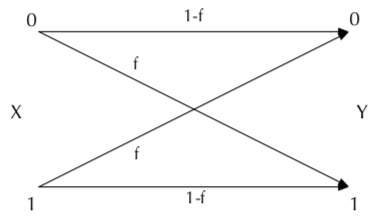
\includegraphics[width=0.5\linewidth, height=4cm]{img/lec17_0}
  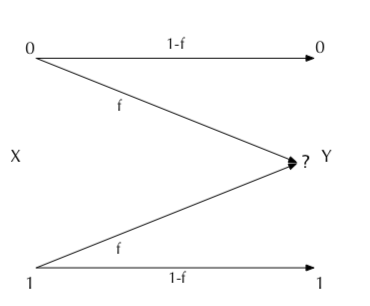
\includegraphics[width=0.5\linewidth, height=4cm]{img/lec17_1}
  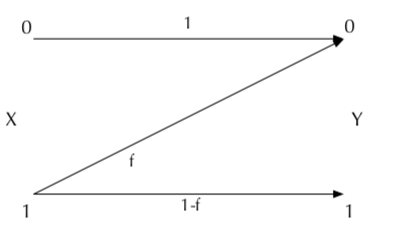
\includegraphics[width=0.5\linewidth, height=4cm]{img/lec17_2}
\end{figure}\\
\newline
\textbf{Channel Capacity- Binary symmetric}\\
**Step 1: Compute H(Y)\\
$q = P_y = Qp_x$:\\
$P(y=0)=(1-f)P(x=0)+fP(X=1)=(1-f)p_0+fp_1$\\
$P(y=1)=p(Y=1|X=1)P(X=1)+p(Y=1|X=0)p(X=0)=(1-f)P(x=1)+fP(X=0)=fp_0+(1-f)p_1$\\
$H(Y) = H_2(q1)=H_2(fp_0+(1-f)p_1)$ when $q=q_1=P(y=1)$\\
**Step 2: Compute $H(Y|X)$\\
$H(Y|X)=\sum H(Y|x)P(x) = \sum_x H_2(f)P(x)=H_2(f)\sum P(x)=H_2(f)$
$I(X;Y) =H(Y)-H(Y|X)=H_2(fp_0+(1-f)p_1)-H_2(f)$ \\
\newline
\textbf{Channel Capacity- non symmetric}\\
I(X;Y) concave in $p_x=(1-p,p)$, single max $\Rightarrow$ stationary point $(I(X;Y))'=0$. If Z channel with $P(y=0|x=1)=f$:\\
$H(Y)=H_2(P(y=1))=H_2(0p_0+(1-f)p_1)=H_2((1-f)p_1)$\\
$H(Y|X)=p_0H_2(P(y=1|x=0))+p_1H_2(P(y=0|x=1))=p_0H_2(0)+p_1H_2(f)$\\
$I(X;Y)=H_2((1-f)p_1)-p_1H_2(f)$\\
$p=\frac{1/(1-f)}{1+2^{H_2(f)/(1-f)}}$\\
\newline
\textbf{Channel Capacity- communication}\\
Message S has a unique block of symbol x with block length N(symbols).\\
(N,K) Block Code: for Q, a list of S=$2^k$ codewords; rate = $\frac{log_2S}{N}=\frac{K}{N}$; rate $\uparrow$, efficient communication$\uparrow$\\
Optimal decoder for code S, channel Q, prior P(s) maps y to output s $P(s|y)$ is maximal.$dec_{opt}(y)= maxP(s|y)=maxP(y|s)P(s)$; y is known.\\

\section{Noisy-Channel Coding Theorem}
If Q is a channel with capacity C then the rate R is achievable if and only if  \\

\section{formulas}
$p(A|B,C)=\frac{p(B|A,C)p(A|C)}{p(B|C)}$\\
$p(A,B,C)=p(C|A,B)*p(B|A)*P(A)=p(C|A,B)*p(A,B)$\\
$p(A,B|C)=p(A|C,B)p(B|C)$\\

\end{document}     